\documentclass{article}
\usepackage{graphicx}
\usepackage{amssymb,amsmath}
\usepackage{tikz}
\usepackage{pgfplots}
\pgfplotsset{compat=newest}
\pgfplotsset{plot coordinates/math parser=false}
\newlength\figureheight
\newlength\figurewidth
\usetikzlibrary{shapes, arrows, patterns}
\usetikzlibrary{external}
\tikzexternalize[shell escape=-enable-write18]
\tikzset{external/system call={lualatex \tikzexternalcheckshellescape -halt-on-error -interaction=batchmode -jobname "\image" "\texsource"}}
\tikzset{external/force remake}

\DeclareRobustCommand{\BlackBox}{\State \textbf{Black Box: }}
\DeclareRobustCommand{\Test}{\State \textbf{Test: }}
\DeclareRobustCommand{\Define}{\State \textbf{Define: }}
\DeclareRobustCommand{\Update}{\State \textbf{Update: }}
\DeclareRobustCommand{\Set}{\State \textbf{Set: }}
\DeclareRobustCommand{\Calculate}{\State \textbf{Calculate: }}
%\newcommand{\algorithmicset}{\textbf{Set:}}
%\algnewcommand\Solve{\item[\algorithmicset]}
%============================================================================
% commands.tex
%============================================================================
% This file contains:
% 	- Defined Variables
%	- Redefined math shorthand
%	- Defined math shorthand


%============================================================================
% Redefined Math Commands
%============================================================================
% 	- \Vec{1} or \vec{1}
%		Long Name: Vector
%		Arguements[1]: bold and overbar arg1	
\DeclareRobustCommand{\Vec}[1]{%
    \ifmmode
        \mathbf{#1}\,%
    \else
        $\displaystyle \mathbf{#1}\,$%
    \fi
}
\DeclareRobustCommand{\vec}[1]{\Vec{#1}}

\DeclareRobustCommand{\lbm}{%
    \ifmmode
        \text{lb}_{\text{m}}
    \else
        $\displaystyle \text{lb}_{\text{m}}$%
    \fi
}
\DeclareRobustCommand{\lbf}{%
    \ifmmode
        \text{lb}_{\text{f}}
    \else
        $\displaystyle \text{lb}_{\text{f}}$
    \fi
}
\DeclareRobustCommand{\dt}{%
	\ifmmode
		\Delta t
	\else
		$\Delta t$
	\fi
}
\DeclareRobustCommand{\dtmax}{%
	\ifmmode
		\Delta t_{\text{MAX}}
	\else
		$\Delta t_{\text{MAX}}$
	\fi
}
\DeclareRobustCommand{\dx}{%
	\ifmmode
		\Delta x
	\else
		$\Delta x$
	\fi
}

\delimitershortfall-1sp
\newcommand\abs[1]{\left|#1\right|}

\tikzstyle{Decision} = [diamond, draw, text width=4.5em, text badly centered, node distance=3cm, inner sep=0pt]
\tikzstyle{Action} = [rectangle, draw,text width=5em, text centered, node distance=3cm, rounded corners, minimum height=0em]
\tikzstyle{NodePoint} = [circle, draw, minimum height = 0 em, node distance = 3 cm]
\tikzstyle{BlackBox} = [rectangle, draw, text centered, node distance=1cm, fill=black!10]
\tikzstyle{line} = [draw, -latex']
    

\begin{document}

\begin{figure}
\centering
\tikzsetnextfilename{images/refillModel_pdf}
{
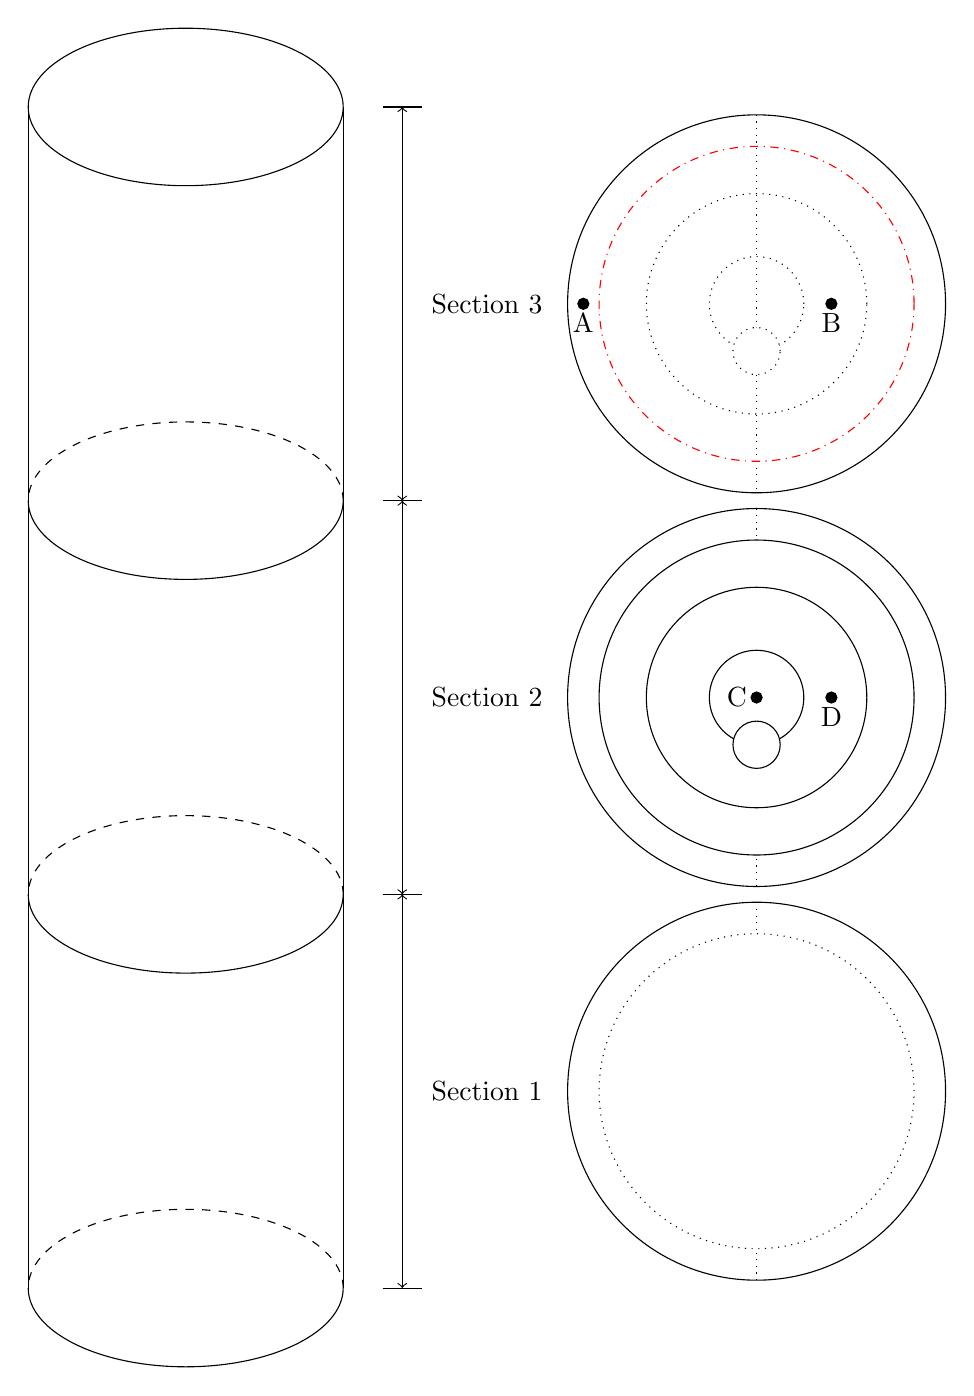
\begin{tikzpicture}

%Boundary Lines
\draw (0,12) circle (2 and 1);
\draw (-2,7) arc (180:360:2 and 1);
\draw [dashed] (2,7) arc (0:180:2 and 1);
\draw (-2,2) arc (180:360:2 and 1);
\draw [dashed] (2,2) arc (0:180:2 and 1);
\draw (-2,-3) arc (180:360:2 and 1);
\draw [dashed] (2,-3) arc (0:180:2 and 1);

%Vertical Lines
\draw (-2,-3) -- (-2,12);
\draw (2,-3) -- (2,12);

%Section 1 Flow Pattern
%\draw (0,9.5) circle (2 and 1);
%\draw [dotted] (0,9.5) circle (1.6 and 0.8);
%\draw (0,9) circle (0.4 and 0.2);
%\filldraw [gray!75] (0.5,9.5) circle (2pt);
%\filldraw [black] (-1.8,9.5) circle (2pt);

%Section 3 Flow Pattern
\draw [dotted] (7.25, 11.9) -- (7.25, 9.2);
\draw [dotted] (7.25, 8.6) -- (7.25, 7.1);
\draw [dotted] (7.25, 9.5) circle (0.6);
\draw [dotted] (7.25, 9.5) circle (1.4);
\draw [dashdotted, color=red]  (7.25, 9.5) circle (2.0);
\draw [solid]  (7.25,9.5) circle (2.4);
\filldraw [dotted, fill=white, draw=black] (7.25, 8.9) circle (0.3);
\filldraw [black] ( 8.2, 9.5) circle (2pt) node[anchor=north]{B};
\filldraw [black] (5.05, 9.5) circle (2pt) node[anchor=north]{A};	

%Section 2 Flow Pattern
\draw [solid] (7.25, 4.5) circle (0.6);
\draw [solid] (7.25, 4.5) circle (1.4);
\draw [solid] (7.25, 4.5) circle (2.0);
\draw [solid] (7.25, 4.5) circle (2.4);
\filldraw [fill=white, draw=black] (7.25, 3.9) circle (0.3);
\draw [dotted] (7.25, 6.9) -- (7.25, 6.5);
\draw [dotted] (7.25, 2.1) -- (7.25, 2.5);
\filldraw [black] (7.25, 4.5) circle (2pt) node[anchor=east]{C};	
\filldraw [black] ( 8.2, 4.5) circle (2pt) node[anchor=north]{D};

%Section 1 Flow Pattern
\draw [solid]  (7.25, -0.5) circle (2.4);
\draw [dotted] (7.25, -0.5) circle (2.0);
\draw [dotted] (7.25,  1.9) -- (7.25,  1.5);
\draw [dotted] (7.25, -2.9) -- (7.25, -2.5);

%Arrows & Labels
\draw (2.5,12) -- (3,12);
\draw [<->] (2.75,12) -- (2.75,7);
\draw (2.5,7) -- (3,7);
\draw [<->] (2.75,7) -- (2.75,2);
\draw (2.5,2) -- (3,2);
\draw [<->] (2.75,2) -- (2.75,-3);
\draw (2.5,-3) -- (3,-3);
\foreach \y/\ytext in {-0.5/Section 1,4.5/Section 2,9.5/Section 3}
	\draw (3,\y) node [anchor=west] {\ytext};

%Extras
\end{tikzpicture}
}
\end{figure}

\end{document}